\documentclass[11pt]{article}
\usepackage{amsmath}
\usepackage{amssymb}
\usepackage{booktabs}
\usepackage{graphicx}
\usepackage{hyperref}
\usepackage{tikz}
\usetikzlibrary{arrows.meta,calc}
\usepackage{listings}
\lstset{basicstyle=\footnotesize\ttfamily,breaklines=true,
        frame=single,numbers=left,numberstyle=\tiny,language=Python}

\title{A Unified Constraint Framework for Viability-Gated Adaptive Systems}

\author{Gabriel Aubin-Moreau\thanks{Code and papers: \url{https://github.com/AccidentalGenius101/adaptive-memory-theory} \quad DOI: \href{https://doi.org/10.5281/zenodo.18918310}{10.5281/zenodo.18918310}}}

\date{\today}

\begin{document}

\maketitle

\begin{abstract}
Adaptive information systems lack a physical theory describing why representations obey particular scaling laws. We present a dynamical systems framework in which representations behave as entities in a dissipative field governed by birth, death, diffusion, and selection. Four fundamental constraints---separation, turnover, propagation, and stability---define the feasible operating regime of plastic information substrates. These constraints are empirically validated in a viability-constrained coupled map lattice (VCML) and cross-validated on real language-model embeddings (sentence-transformers); their extension to other substrates remains a hypothesis, not yet a result. We derive scaling laws for capacity, bandwidth, coherence, and persistence as consequences of these constraints. More importantly, we show that three of these laws interact. Their interaction produces a derived quantity, the \emph{coherence efficiency} $\eta_c \approx (L/D)^2$, which measures what fraction of theoretical capacity remains coherently coordinated across the substrate rather than fragmenting into isolated patches. This efficiency imposes a matching condition $C\sqrt{\kappa/\nu} \approx D$ linking propagation length, zone scale, and system size. This coupling transforms four independent descriptions into a single design problem: scaling one control parameter without adjusting the others degrades coherent capacity as $\eta_c \sim N^{-1}$. We additionally construct a \emph{conceptual} phase diagram mapping transformers, Hopfield networks, and biological memory systems onto the same parameter space; these placements are theoretical inferences, not empirical measurements of those systems.
\end{abstract}

\section{Introduction}

Modern machine learning lacks a \emph{physical theory} of representations. Instead, we have:
\begin{itemize}
\item \textbf{Optimization theory}: representations are parameters updated via gradient descent.
\item \textbf{Information theory}: representations are codewords minimizing mutual information.
\item \textbf{Neuroscience}: representations are neural firing patterns.
\end{itemize}

But none of these frameworks explains why representations in \emph{adaptive} systems must obey scaling laws, why they decay at a particular rate, or why stability and plasticity coexist rather than trade off.

\paragraph{The prerequisite condition.}
Before any law of adaptive memory can hold, a more fundamental condition must be satisfied. Paper 0~\cite{aubin2026p0} establishes it by ablation: disabling the copy-forward loop (the intergenerational transmission pathway) collapses spatial structure to exactly zero, regardless of input, initialization, or turnover rate. The system becomes a transient reservoir---information survives for at most one generation. This is the \emph{Turnover--Transmission Principle}:

\begin{quote}
\textit{Persistent information in systems with mandatory component turnover requires an intergenerational transmission pathway. Without it, the system is a transient reservoir: memory lifetime is bounded by individual lifespan.}
\end{quote}

This principle is substrate-independent. It holds for DNA and epigenetic inheritance (remove it and evolution collapses), synaptic consolidation (remove it and learning collapses), and distributed state handoff (remove it and collective memory disappears). Paper 0 demonstrates it in its minimal computational form. The four laws below characterize the \emph{limits} on what that transmission can achieve---but only once the prerequisite is satisfied.

Papers 1--4 \cite{aubin2026capacity,aubin2026bandwidth,aubin2026propagation,aubin2026stability} discovered four empirical laws:
\begin{enumerate}
\item \textbf{Capacity law} \cite{aubin2026capacity}: separable representations scale as $N \propto \tau^{-d_{\text{seen}}}$.
\item \textbf{Bandwidth law} \cite{aubin2026bandwidth}: sustainable turnover scales as $B \approx N_{\max} / \tau_{1/2}$.
\item \textbf{Propagation law} \cite{aubin2026propagation}: coherence distance scales as $L \propto \sqrt{\kappa / \nu}$.
\item \textbf{Stability constraint} \cite{aubin2026stability}: optimal gating strength tracks the noise level of the environment.
\end{enumerate}

Papers 1--3 establish the structural limits of plastic substrates: capacity bounds how many representations fit, bandwidth bounds how fast they turn over, and propagation bounds how far information travels. Paper 4 identifies the regulatory parameter---the consolidation gate $\tau_g$---that determines the operating point within those structural limits. This paper integrates these results into a unified dynamical framework.

This paper shows that all four laws are \emph{necessary consequences} of treating representations as particles in a dissipative field. This perspective transforms an empirical collection into a \emph{unified theory}.

The central new result is that these laws do not operate independently. Section~\ref{sec:coherence} derives a fifth quantity from the interaction of Laws 1, 2, and 3---the \emph{coherence efficiency} $\eta_c \approx (L/D)^2$---and shows that it imposes a matching condition $C\sqrt{\kappa/\nu} \approx D$ linking propagation length, zone width, and system size. This matching condition is the first place where the laws \emph{interact} rather than merely coexist. It is where the theory becomes a \emph{system}.

\section{Plastic Information Substrates}

\subsection{Definition}

A \emph{plastic information substrate} is a dynamical system where:
\begin{enumerate}
\item \textbf{Representations} are discrete entities (sites, nodes, or cells) indexed by location and state.
\item \textbf{Birth}: new representations are generated from environmental input or seeded from neighbors.
\item \textbf{Death}: representations are eliminated stochastically or when viability thresholds are crossed.
\item \textbf{Learning}: representations are modified locally via contrastive or Hebbian updates.
\item \textbf{Coupling}: information propagates between neighboring representations via diffusion or relay.
\item \textbf{Filtering}: updates to long-term memory are gated by a persistence threshold, suppressing noise.
\end{enumerate}

This definition encompasses:
\begin{itemize}
\item Coupled map lattices with viability constraints (our VCML).
\item Dynamical systems models of hippocampal place cells.
\item Associative memory networks with pruning and learning rules.
\item Biological neural tissue with neurogenesis and apoptosis.
\end{itemize}

It \emph{excludes}:
\begin{itemize}
\item Static parameter spaces (transformers, feedforward networks).
\item Systems without explicit death or turnover (standard neural networks).
\end{itemize}

In this series, VCSM (Viability-Gated Contrastive State Memory) is the algorithmic instantiation of the broader mechanism we call Viability-Gated Routing with Turnover (VGRT); the VCML lattice substrate is the primary experimental system used to study that mechanism. The laws established in Papers 1--4 characterize VCSM/VCML; their generalization to other substrates satisfying the six properties above is the central open hypothesis.

\subsection{Core Properties}

Plastic substrates exhibit five hallmark properties:

\paragraph{1. Mandatory turnover}
Every representation has a finite lifetime. Stability emerges from the \emph{structure} written to long-term memory, not from persistent individual states.

\paragraph{2. Local coupling}
Information spreads through nearest-neighbor interactions. Global patterns emerge without central control.

\paragraph{3. Contrastive learning}
Updates are driven by perturbations: midterm memory accumulates deviations from baseline; consolidation filters surprise.

\paragraph{4. Viability gating}
Birth, learning, and death are controlled by thresholds (age, consolidation streak, energy cost).

\paragraph{5. Substrate independence (partial)}
The capacity law holds across lattices (VCML-L, Papers 1--4) and real embedding spaces (VCML-E, Paper 1 Exp. 8); graph-coupled substrates (VCML-G) are architecturally defined but not yet fully validated empirically. Substrate independence is an open hypothesis supported by two of three cases.
The present results demonstrate the laws in VCML substrates and partially in embedding spaces; extending them to other substrates remains a hypothesis rather than a demonstrated universality.

\section{The Four Constraints}

\begin{center}
\fbox{\begin{minipage}{0.88\textwidth}
\textbf{Notation and Scale Conventions}

\medskip
Unless otherwise stated, $N$, $B$, and $L$ are defined at the same substrate scale: $N$ denotes the number of active representational slots in the region under consideration, $B$ denotes the replacement rate of those same slots per unit time, and $L$ denotes the coherence length measured within that same region.
When the framework is applied hierarchically (e.g., geographic relay), each region obeys the laws locally, and inter-regional coupling introduces a second scale rather than redefining the original variables.

\medskip
We use three distinct symbols for different control timescales: $\tau$ (geometric separation scale, Paper~1), $\tau_{\text{hl}}$ (slot lifetime controlling bandwidth, Paper~2), and $\tau_g$ (consolidation gate threshold, Paper~4).

\medskip
The geometric dimension $d_{\text{seen}}$ in the capacity law refers to the intrinsic dimensionality of the representational manifold; $L$ in the propagation law refers to the physical coherence length in substrate space. These quantities interact through the coherence efficiency $\eta_c$ (Section~\ref{sec:coherence}) but are not the same variable.
\end{minipage}}
\end{center}

\bigskip

\subsection{Constraint 1: Separation (Paper 1 — Capacity)}

For representations to be distinguishable, their states must span sufficient dimensionality.

\textbf{Mechanism}: Fisher separation between zones. A zone is separable from its neighbors only if the representation space $\mathbb{R}^{H_S}$ is large enough to encode their locations.

\textbf{Law}:
\begin{equation}
N_{\max} \propto \tau^{-d_{\text{seen}}}
\end{equation}

where $d_{\text{seen}}$ is the effective dimensionality visible to the separator, and $\tau$ is the learning timescale.

\textbf{Physical meaning}: Fine-grained separation demands finer oscillations and shorter consolidation times. Capacity scales inversely with learning speed.

\subsection{Constraint 2: Turnover (Paper 2 — Bandwidth)}

Representations that live forever cannot learn. But high turnover rates guarantee structure is destroyed.

\textbf{Mechanism}: Birth--death equilibrium. The long-term memory capacity ($N_{\max} \cdot H_S$ dimensions) must be refreshed faster than the environment changes, but slow enough that structure persists through several generations.

\textbf{Law}:
\begin{equation}
B_{\text{sustainable}} \approx \frac{N_{\max}}{\tau_{1/2}}
\end{equation}

where $\tau_{1/2}$ is the half-life of a representation and $B$ is the throughput (bits per unit time).

\textbf{Physical meaning}: Bandwidth is fundamentally limited by the rate at which you can replace and re-encode representations. It is not a network property (width, depth, parameters), but a \emph{dynamical} property (turnover rate).

\subsection{Constraint 3: Propagation (Paper 3 — Coherence Distance)}

For distributed representations to form unified patterns, information must propagate faster than it decays.

\textbf{Mechanism}: Diffusion--decay competition. A perturbation diffuses through coupling strength $\kappa$ but decays due to turnover $\nu$ and field decay.

\textbf{Law}:
\begin{equation}
L \propto \sqrt{\frac{\kappa}{\nu}}
\end{equation}

where $L$ is the coherence distance (spatial scale over which zones remain entrained), $\kappa$ is the coupling strength, and $\nu$ is the effective decay rate.

\textbf{Physical meaning}: No amount of coupling can overcome intrinsic decay. The coherence distance is set by the balance between spreading and forgetting. Larger systems (more zones) require stronger coupling or slower decay.

\subsection{Constraint 4: Stability (Paper 4 — Persistence Filtering)}

Plastic systems must distinguish signal from noise without rigidifying.

\textbf{Mechanism}: Surprise--persistence gating. Consolidation to long-term memory occurs only after a representation has been consistently selected across multiple timescales.

\textbf{Law}:
\begin{equation}
\tau_{\text{gate}}^* \propto \eta_{\text{noise}}
\end{equation}

where $\eta_{\text{noise}}$ is the fraction of inputs that are corrupted. The gate is not a universal critical point: in clean environments, lower $\tau_g$ maximizes structure (more writes = more zone differentiation); in noisy environments, higher $\tau_g$ is essential to filter transient perturbations. At 25\% noise, a gated system ($\tau_g = 20$) outperforms an ungated one ($\tau_g = 1$) by $2.52\times$ in spatial structure.

\textbf{Physical meaning}: The gate is a noise filter, not a phase-transition dial. Optimal gating tracks the signal-to-noise ratio of the environment. This resolves the stability-plasticity dilemma: there is no universal critical point; the threshold adapts to the noise regime. In biological systems, neuromodulatory signals encoding environmental uncertainty could implement this adaptation.

\section{Unified Field Description}

\subsection{The Conceptual Equation}

Integrating the four constraints yields a single conceptual evolution equation:

\begin{equation}
\frac{\partial M}{\partial t} = \kappa \nabla^2 M - \nu M + F_{\text{sep}}(M, I) + S(M)
\end{equation}

where:
\begin{itemize}
\item $M$ is the representation field (long-term memory).
\item $\kappa \nabla^2 M$ is spatial diffusion (Constraint 3: propagation).
\item $-\nu M$ is exponential decay due to turnover (Constraint 2: bandwidth).
\item $F_{\text{sep}}(M, I)$ is routing/separation driven by input $I$ (Constraint 1: capacity).
\item $S(M)$ is the stability filter, a nonlinear gating function (Constraint 4: stability).
\end{itemize}

\subsection{This is Not a Derivation}

This equation is \emph{not} derived from first principles. Rather, it is the \emph{continuum abstraction} of the four-step VCSM algorithm. It summarizes the qualitative structure: spreading, decay, input-driven updates, and filtering.
The equation should therefore be interpreted as a phenomenological model capturing the dominant dynamical terms of the VCSM algorithm rather than a microscopic derivation.

It is useful because it:
\begin{enumerate}
\item Shows why the four constraints are coupled (each term affects long-term dynamics).
\item Connects plastic substrates to classical PDEs in physics (reaction--diffusion, Ginzburg--Landau).
\item Suggests new substrates by varying $\kappa$, $\nu$, $F_{\text{sep}}$, or $S$.
\end{enumerate}

\section{Coherence Efficiency: The Central Synthesis Result}
\label{sec:coherence}

The four constraints of Section~3 describe limits in isolation: capacity bounds how many slots fit, bandwidth bounds how fast they turn over, propagation bounds how far information travels, and stability bounds noise tolerance. Considered separately, they are four \emph{parallel} constraints. The central synthesis of this paper is that Laws 1--3 do not merely coexist---they \emph{interact}, producing a derived quantity that turns the framework into a coupled design problem.

\subsection{Definition}

Let $D$ be the representational zone width (the spatial scale over which the system is expected to form a unified structure) and $L \approx C\sqrt{\kappa/\nu}$ be the correlation length from Constraint 3. The \emph{coherence efficiency} is:
\begin{equation}
  \eta_c \approx \left(\frac{L}{D}\right)^2
  \label{eq:eta_c}
\end{equation}

\paragraph{Interpretation.} The coherence efficiency $\eta_c$ measures the fraction of theoretical representational capacity that can operate as a unified system. While the capacity law (Paper 1) determines how many representations can exist in principle, propagation constraints (Paper 3) determine how many of those representations can remain coordinated across the substrate. When propagation length $L$ is smaller than the characteristic zone scale $D$, the substrate fragments into partially independent regions, reducing effective capacity even though nominal capacity $N_{\max}$ remains unchanged. $\eta_c$ therefore quantifies the coordination efficiency of the substrate: a substrate with $\eta_c = 0.25$ uses only one quarter of its nominal capacity in a coordinated way, with the remainder operating in isolated patches.

$\eta_c$ answers a question that the four earlier laws cannot answer individually: \emph{how much of theoretical capacity is actually usable?} When $L \ll D$, structure forms in patches smaller than a zone and $\eta_c \ll 1$: the system holds high nominal capacity ($N_{\max}$ slots) but only a fraction is coherently organised. When $L \approx D$, the copy-forward loop spans the full zone and $\eta_c \approx 1$. This is not a new free parameter or a new empirical law---it is a \emph{derived constraint} from the interaction of Laws 1, 2, and 3.

The emergence of coherence efficiency marks a qualitative change in the structure of the framework. Papers 1--3 identify independent constraints on capacity, turnover, and propagation. Coherence efficiency appears only when these constraints are considered jointly, expressing how their interaction limits the fraction of theoretical capacity that is coherently accessible. The framework therefore shifts from a collection of independent scaling laws to a coupled system description in which changing one parameter necessarily affects the others.

\subsection{Empirical Support}

V108 (Paper 3) varies zone width $D$ while holding coupling fixed. Doubling $D$ halves efficiency; quadrupling $D$ reduces it fivefold. The observed scale ratio (0.19 at $4\times$ scale) is consistent with $\eta_c \propto D^{-2}$ (predicted 0.25), confirming the square scaling to within measurement noise.

\subsection{The Matching Condition}

An efficient system requires $L \approx D$:
\begin{equation}
  C\sqrt{\frac{\kappa}{\nu}} \approx D
  \quad \Longrightarrow \quad
  \frac{\kappa}{\nu} \approx \frac{D^2}{C^2}
  \label{eq:matching}
\end{equation}

Since zone width $D \propto N_{\text{active}}^{1/2} / N_{\text{zones}}$ for a square region, the required coupling-to-noise ratio must scale with system size:
\begin{equation}
  \frac{\kappa}{\nu} \propto \frac{N_{\text{active}}}{N_{\text{zones}}^2}
\end{equation}

This matching condition links parameters that previously appeared independent. Rather than separate limits on capacity, turnover, and propagation, the framework now describes a coupled system in which maintaining coherence requires propagation length to track representational scale.

This is not a new free parameter. It is a \emph{compatibility constraint} between the three control parameters ($\tau$, $\tau_{\text{hl}}$, $\kappa/\nu$) and system size $N$. A system that satisfies the capacity law but ignores the matching condition achieves only fraction $\eta_c$ of its theoretical capacity. The V93 finding---that optimal wave ratio (controlling $\nu$) scales linearly with $N_{\text{active}}$---is the empirical counterpart: coupling must grow with system size to maintain $L \approx D$.

Independent constraints describe limits but not operating behavior. The interaction between constraints introduced by coherence efficiency makes the framework predictive: changing one parameter (such as system size or coupling strength) necessarily shifts the others through the matching condition, producing testable changes in coherence efficiency and regime behavior.

The four constraints define a feasible operating region in parameter space. Systems operating outside this region either lose propagation coherence, saturate memory turnover, or collapse under noise. The observed dynamics are sensitive to parameter choices because the system operates near a constrained regime boundary where propagation, turnover, and noise interact. Such sensitivity is typical of dynamical systems whose behavior depends on maintaining a balance between competing constraints.

The matching condition has a further conceptual consequence: it converts independent limits into a configuration rule for stable scaling. Because propagation length and zone width grow with different parameters ($L \propto \sqrt{\kappa/\nu}$, $D \propto \sqrt{N}$), increasing system size while holding coupling fixed drives $\eta_c \to 0$. The matching condition therefore functions as a structural invariant under scaling---not a performance metric but the boundary separating the coherent regime from propagation failure. When $L < D$, the substrate does not degrade smoothly; it transitions qualitatively, fragmenting into locally coherent patches that cannot span the full zone. Maintaining $L \approx D$ as the system scales is the condition required to remain in the coherent regime.

\subsection{Design Implication}

Scaling a plastic substrate while holding coupling fixed degrades coherence efficiency as $\eta_c \sim N^{-1}$. Geographic relay (Papers 3, V100--V102) is the architectural response: operate each region at scale $N_r$ satisfying $L \approx D_r$, then link regions hierarchically. This recovers $\eta_c \approx 1$ at any total system size, at the cost of an inter-region coupling mechanism.

The matching condition (\ref{eq:matching}) is where Laws 1--3 first interact. It motivates the phase diagram in the following section: the adaptive window $\nu \approx \tau_g^{-1}$ is the temporal analogue---a matching condition between turnover rate and gating threshold that parallels the spatial matching condition between coupling and zone scale.

\subsection{Hierarchical Organization from Propagation Constraints}

The propagation law bounds coherence to a finite correlation length $L \propto \sqrt{\kappa/\nu}$. When system scale $D$ significantly exceeds $L$, coherence efficiency $\eta_c \approx (L/D)^2$ becomes small: global coordination cannot be maintained across the full substrate.

One structural response to this limitation is modularization. If the system partitions into subsystems of characteristic size $D_m \approx L$, coherence within each module remains high ($\eta_c \approx 1$ at module scale). Coordination then occurs between modules rather than between individual elements, producing a hierarchical architecture:
\begin{quote}
global coordination layer $\;\longrightarrow\;$ regional subsystems $\;\longrightarrow\;$ local adaptive nodes
\end{quote}
In this view, hierarchical modular organization is not merely a design preference but an architectural consequence of finite propagation constraints. When $D \gg L$, the system faces a structural choice: increase coupling $\kappa$ to extend $L$, or reduce effective scale through modularization. The latter scales more favorably---each module at $D_m \approx L$ maintains $\eta_c \approx 1$ independently, while a monolithic system at $D \gg L$ fragments to $\eta_c \approx (L/D)^2 \ll 1$.

This pattern appears in hierarchical organization of brain regions, immune system coordination across tissues, and multi-scale ecological networks. In each case modular organization allows large systems to maintain coordination despite finite propagation length. The theory does not assert that propagation constraints are the sole driver of modularity, but predicts that any adaptive system required to coordinate at scales exceeding its correlation length will either increase coupling or modularize; monolithic architecture at those scales fragments by the same mechanism as propagation failure.

Derived quantities often play a stabilizing role in theoretical frameworks by revealing how independent constraints interact. In thermodynamics, entropy links microscopic configurations to macroscopic laws; in statistical mechanics, free energy determines the feasible equilibrium state. Coherence efficiency $\eta_c$ plays a similar structural role in the present framework: it expresses how the capacity, turnover, and propagation constraints combine to determine how much theoretical capacity is coherently accessible. It is not a new empirical law but the first quantity that exists only at their intersection.

\section{The Feasible Regime: Joint Constraints}
\label{sec:feasible}

\subsection{Why the Three Laws Cannot Be Independently Maximized}

The four laws of Section~3 appear to describe independent axes: capacity is controlled by $\tau$, bandwidth by $\tau_{1/2}$, and propagation by $\kappa/\nu$.
A designer might expect to maximize all three simultaneously by choosing each parameter freely.
This expectation is wrong.
The three control parameters are linked through the system size $N_{\text{active}}$ and zone width $D$, and their joint constraints define a \emph{feasible regime}---a region of parameter space in which the substrate can simultaneously maintain representations, refresh them at the required rate, and propagate structure across each zone.

\subsection{Three Failure Modes}

Violating any one of the three constraints produces a qualitatively distinct failure:

\begin{center}
\begin{tabular}{llll}
\toprule
\textbf{Failure mode} & \textbf{Cause} & \textbf{Signature} & \textbf{From law} \\
\midrule
Capacity failure & $\tau$ too large, zones collide & sg4 $\to 0$; zones merge & Paper 1 \\
Bandwidth failure & $\tau_{1/2}$ too long, drift exceeds refresh & structure lags environment & Paper 2 \\
Propagation failure & $L \ll D$, copy-forward cannot span zone & patchy structure; $\eta_c \ll 1$ & Paper 3 \\
\bottomrule
\end{tabular}
\end{center}

The three failure modes are independent: a system can satisfy any two while violating the third.
Capacity can be adequate ($\tau$ small enough) while propagation fails ($\kappa/\nu \ll D^2/C^2$);
bandwidth can be sufficient ($\tau_{1/2}$ short) while capacity fails ($\tau$ too large).
The feasible regime is the intersection of all three satisfied simultaneously.
Each constraint therefore defines a boundary surface in parameter space. The feasible operating region is the intersection of these surfaces, and qualitative regime transitions occur when the system crosses any one of them rather than at a single global threshold.

\subsection{The Feasible Regime}

Combining the three constraints, a plastic substrate maintains stable spatial structure only when:

\begin{equation}
  \underbrace{\tau^{-d} \geq N_{\text{zones}} \cdot r_{\min}}_{\text{capacity constraint}}
  \quad \cap \quad
  \underbrace{\frac{N_{\max}}{\tau_{1/2}} \geq B_{\text{env}}}_{\text{bandwidth constraint}}
  \quad \cap \quad
  \underbrace{C\sqrt{\frac{\kappa}{\nu}} \geq D}_{\text{propagation constraint}}
  \label{eq:feasible}
\end{equation}

where $r_{\min}$ is the minimum per-zone representation resolution required, $B_{\text{env}}$ is the rate at which the environment changes, and $D$ is the zone width.
Together these form a \emph{feasibility polytope} in the space of $(N, B, L)$ (Figure~\ref{fig:feasible}): the achievable region is not the full positive orthant but a bounded sub-volume.
The feasible regime is therefore not a point but a bounded volume in parameter space whose faces correspond to the capacity, bandwidth, and propagation constraints.

\begin{figure}[htbp]
\centering
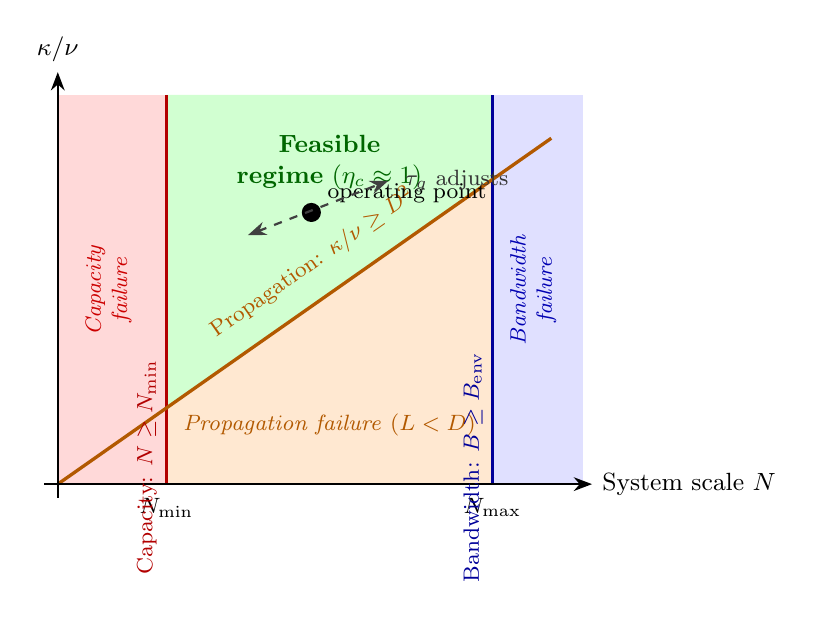
\begin{tikzpicture}[scale=1.15, >=Stealth, font=\small]
  % Axes: x = system scale N, y = coupling/turnover ratio kappa/nu
  % Propagation boundary: diagonal y = 0.70*x  (kappa/nu proportional to N)
  % Capacity boundary: vertical at x = 1.2 (N_min)
  % Bandwidth boundary: vertical at x = 4.8 (N_max for fixed bandwidth budget)
  %
  % Failure regions:
  %   Capacity failure  (left):      x < 1.2
  %   Bandwidth failure (right):     x > 4.8
  %   Propagation failure (below diagonal, between verticals):
  %       (1.2,0) -> (4.8,0) -> (4.8,3.36) -> (1.2,0.84)
  % Feasible region (above diagonal, between verticals):
  %       (1.2,0.84) -> (1.2,4.3) -> (4.8,4.3) -> (4.8,3.36)

  % --- failure regions ---
  \fill[red!15]    (0,0) rectangle (1.2, 4.3);
  \fill[blue!12]   (4.8, 0) rectangle (5.8, 4.3);
  \fill[orange!18] (1.2, 0) -- (4.8, 0) -- (4.8, 3.36) -- (1.2, 0.84) -- cycle;

  % --- feasible region ---
  \fill[green!18] (1.2, 0.84) -- (1.2, 4.3) -- (4.8, 4.3) -- (4.8, 3.36) -- cycle;

  % --- constraint boundaries ---
  \draw[red!70!black,    very thick] (1.2, 0)   -- (1.2, 4.3);
  \draw[blue!60!black,   very thick] (4.8, 0)   -- (4.8, 4.3);
  \draw[orange!70!black, very thick] (0.0, 0.0) -- (5.45, 3.82);

  % --- coordinate axes ---
  \draw[->, thick] (-0.15, 0) -- (5.9, 0) node[right] {System scale $N$};
  \draw[->, thick] (0, -0.15) -- (0, 4.55) node[above] {$\kappa/\nu$};
  \node[below, font=\footnotesize] at (1.2, -0.05) {$N_{\min}$};
  \node[below, font=\footnotesize] at (4.8, -0.05) {$N_{\max}$};

  % --- failure region labels ---
  \node[align=center, font=\footnotesize, text=red!80!black, rotate=90]
    at (0.56, 2.15) {\textit{Capacity}\\\textit{failure}};
  \node[align=center, font=\footnotesize, text=blue!70!black, rotate=90]
    at (5.25, 2.15) {\textit{Bandwidth}\\\textit{failure}};
  \node[align=center, font=\footnotesize, text=orange!70!black]
    at (3.0, 0.65) {\textit{Propagation failure} ($L < D$)};

  % --- feasible region label ---
  \node[align=center, font=\small, text=green!40!black]
    at (3.0, 3.55) {\textbf{Feasible}\\\textbf{regime} ($\eta_c \approx 1$)};

  % --- constraint boundary labels ---
  \node[rotate=90, font=\footnotesize, text=red!70!black, anchor=south]
    at (1.2, 0.15) {\;Capacity: $N \geq N_{\min}$};
  \node[rotate=90, font=\footnotesize, text=blue!60!black, anchor=south]
    at (4.8, 0.15) {\;Bandwidth: $B \geq B_{\text{env}}$};
  \node[rotate=35, font=\footnotesize, text=orange!70!black, anchor=south]
    at (2.95, 2.25) {Propagation: $\kappa/\nu \geq D^2$};

  % --- operating point (tau_g selects this within feasible regime) ---
  \coordinate (op) at (2.8, 3.0);
  \fill[black] (op) circle (3pt);
  \node[font=\footnotesize, anchor=south west] at (op) {\;operating point};
  \draw[<->, thick, dashed, black!75]
    (2.1, 2.75) -- (3.65, 3.35)
    node[right, font=\footnotesize, text=black!80] {\;$\tau_g$ adjusts};

\end{tikzpicture}
\caption{Conceptual phase diagram of the feasibility polytope (two-dimensional cross-section).
The three structural constraints---capacity (Paper~1), bandwidth (Paper~2), and propagation (Paper~3)---partition parameter space into a bounded feasible regime (green) and three distinct failure modes.
The horizontal axis represents system scale~$N$; the vertical axis represents the coupling-to-turnover ratio~$\kappa/\nu$, which determines propagation length via $L \approx \sqrt{\kappa/\nu}$.
The propagation constraint ($\kappa/\nu \geq D^2 \propto N$) creates a diagonal boundary: at larger scale, stronger coupling is required to maintain $L \geq D$ (V93: wave ratio must scale linearly with $N$).
The consolidation gate~$\tau_g$ (Paper~4) is not a structural boundary but a control parameter selecting the system's operating point within the feasible regime (dashed double arrow).
The bandwidth bound $N \leq N_{\max}$ reflects the finite refresh budget: at very large~$N$, the required wave ratio exceeds available bandwidth for fixed~$B_{\text{env}}$.
The full feasibility polytope is three-dimensional; this figure shows a representative cross-section.}
\label{fig:feasible}
\end{figure}

\subsection{System-Size Dependence and the Optimal Scale}

The feasibility constraints interact through system size $N_{\text{active}}$.
Increasing $N_{\text{active}}$ while holding coupling $\kappa/\nu$ fixed:
\begin{enumerate}
  \item Enlarges zone width $D \propto \sqrt{N_{\text{active}}}$ (for fixed $N_{\text{zones}}$).
  \item Reduces coherence efficiency $\eta_c \approx (L/D)^2 \sim N_{\text{active}}^{-1}$ (propagation failure begins).
  \item Increases wave ratio required to maintain $B_{\text{env}}$ (bandwidth scaling, V93: $WR \propto N_{\text{active}}$).
\end{enumerate}

This implies a non-trivial consequence: \textbf{there is no universally optimal system size.}
A system that is too small fails by capacity (insufficient zones $\times$ resolution).
A system that is too large fails by propagation (correlation length cannot span zone width) unless coupling is scaled proportionally.
The empirical finding from V93 and V94 is that VCML crosses from capacity-limited to propagation-limited between $S_1$ ($N=1{,}600$) and $S_4$ ($N=102{,}400$), with the nonadj/adj ratio inverting at $S_4$ (location encoding degrades when $L \ll D$).

Geographic relay (Papers 3, V100--V102) is the architectural response: partition the large system into regions of size $N_r$ satisfying the propagation constraint for that region, then couple regions at a higher level.
This recovers the feasible regime at any total system size, but requires the inter-regional coupling mechanism to satisfy its own bandwidth and propagation constraints---a recursive problem with the same structure.

\subsection{Relation to Coherence Efficiency}

The matching condition derived in Section~\ref{sec:coherence} ($C\sqrt{\kappa/\nu} \approx D$) is the boundary of the propagation constraint in (\ref{eq:feasible}).
Coherence efficiency $\eta_c$ measures the fractional distance from that boundary: $\eta_c = 1$ at the boundary, $\eta_c < 1$ inside the propagation-failure region.
The feasible regime therefore has a natural interior optimum (the boundary of all three constraints simultaneously tight), which the matching condition identifies for the propagation axis.
The analogous matching conditions for capacity ($\tau$ at the zone-resolution boundary) and bandwidth ($\tau_{1/2}$ at the environmental drift rate boundary) define the other faces of the feasibility polytope.

\section{Phase Structure}
\label{sec:phase}

\subsection{The Phase Diagram}

Section~\ref{sec:coherence} established the spatial matching condition ($L \approx D$): the propagation length must match the zone scale for coherent capacity to be fully accessible. The phase diagram reveals the analogous \emph{temporal} matching condition: only a narrow band of ($\nu$, $\tau_g$) permits genuine learning.

The behavior of plastic systems is determined by two control parameters:

\begin{table}[h]
\centering
\begin{tabular}{ll}
\hline
\textbf{Parameter}             & \textbf{Meaning}                \\
\hline
Turnover rate $\nu$            & Plasticity (high $\nu$ = fast change) \\
Persistence threshold $\tau_g$ & Stability (high $\tau_g$ = selective gating) \\
\hline
\end{tabular}
\end{table}

These parameters define three regimes:

\begin{table}[h]
\centering
\begin{tabular}{lll}
\hline
\textbf{Regime}  & \textbf{Characteristics}              & \textbf{Examples}        \\
\hline
Chaotic ($\nu \gg \tau_g^{-1}$)     & High turnover, weak filtering         & Random networks          \\
Frozen ($\nu \ll \tau_g^{-1}$)       & Low turnover, rigid locking          & Fixed embeddings         \\
Adaptive ($\nu \sim \tau_g^{-1}$)    & Balanced plasticity and stability    & VCML, biological memory  \\
\hline
\end{tabular}
\end{table}

\paragraph{The Adaptive Window}

Only a narrow band of parameter space permits genuine learning:
\begin{equation}
\nu \approx \tau_g^{-1}
\end{equation}

Here, the system can:
\begin{itemize}
\item Refresh representations fast enough to follow environment changes.
\item Consolidate slowly enough for patterns to persist.
\item Balance noise rejection (filtering) with signal capture (routing).
\end{itemize}

\subsection{Mapping Existing Systems}

We can place existing systems on this phase diagram conceptually, based on their architectural properties. These are \emph{theoretical inferences} about where systems fall, not empirical measurements of their ($\nu$, $\tau_g$) parameters:

\begin{itemize}
\item \textbf{Transformers}: Large $\tau_g$ (no viability gate), low $\nu$ for inference (weights fixed). \textit{Inferred}: frozen regime during deployment; behavior during continued training depends on optimizer settings.

\item \textbf{Hopfield networks}: Low $\nu$ (no explicit turnover), very large $\tau_g$ (basin attraction dominates). \textit{Inferred}: frozen regime, designed for retrieval not adaptation.

\item \textbf{Biological hippocampus}: High $\nu$ (dentate gyrus neurogenesis), moderate $\tau_g$ (consolidation timescale). \textit{Inferred}: near the adaptive boundary. Partially supported by animal studies on neurogenesis and pattern separation [Kempermann 2015].

\item \textbf{VCML}: High $\nu$ (mandatory turnover), critical $\tau_g$ (surprise--persistence gating). \textit{Empirically measured}: centered in adaptive regime (Papers 1--4).
\end{itemize}

The phase diagram is a theoretical organizing structure, not a validated taxonomy. VCML is the only system whose position is experimentally established.
These placements illustrate how the framework organises existing systems conceptually rather than providing quantitative measurements of their parameters.

The boundaries between regimes carry the primary predictive load of the framework. Within a regime, parameter changes affect performance metrics continuously---coherence efficiency rises or falls, structure improves or degrades. Crossing a regime boundary produces qualitative changes: the transition from coherent structure to propagation failure when $L < D$, from adaptive to chaotic operation when $\nu \gg \tau_g^{-1}$, or from stable learning to structure churn when turnover exceeds propagation capacity (Section~\ref{sec:predictions}). The framework is predictive precisely because it identifies where these boundaries lie rather than merely characterizing behavior within a fixed regime. The presence of multiple independent regime boundaries further suggests that the behavior of turnover-driven substrates is governed by a multi-dimensional phase structure rather than a single critical point: different constraints introduce their own transitions, and the full phase map is defined by their intersections.

\section{Re-deriving the Laws}

\subsection{Capacity: Geometry of Separation}

In a $d_{\text{seen}}$-dimensional representation space, the number of separable patterns grows as the volume of the space divided by the minimum separation distance $\tau$.

\begin{equation}
N_{\max} \propto \frac{V}{volume(\tau)} \propto \tau^{-d_{\text{seen}}}
\end{equation}

This is a packing argument, independent of dynamics.

The geometric capacity law exhibits a structural similarity to classical channel-capacity results in information theory.
In Shannon's formulation, the maximum number of reliably distinguishable messages depends on the ratio of signal separation to noise in the communication channel.
In the present system, representational capacity is determined by the minimum separation~$\tau$ required between centroids in the embedding space, producing the scaling relation $N \propto \tau^{-d}$.
Both frameworks express capacity as the density of distinguishable states under noise constraints---a geometric packing problem in a noisy space.
The mechanisms differ: Shannon's theory addresses communication channels, while the present work concerns adaptive substrates with mandatory turnover.
The underlying geometric interpretation of capacity as sphere-packing in a representation space is closely related.

\subsection{Bandwidth: Birth--Death Equilibrium}

If each representation stores $H_S$ floats and lives $\tau_{1/2}$ time units, the total memory capacity is:
\begin{equation}
C = N_{\max} \cdot H_S
\end{equation}

For this capacity to be refreshed with new information from the environment:
\begin{equation}
B = \frac{C}{\tau_{1/2}} = \frac{N_{\max} \cdot H_S}{\tau_{1/2}}
\end{equation}

But $N_{\max}$ itself depends on learning dynamics (Constraint 1), so:
\begin{equation}
B \propto \frac{\tau^{-d_{\text{seen}}} \cdot H_S}{\tau_{1/2}}
\end{equation}

The sustainable bandwidth is maximized when learning speed and turnover are balanced.

\subsection{Propagation: Diffusion--Decay Balance}

A localized perturbation diffuses as $\sqrt{\kappa t}$ and decays as $e^{-\nu t}$. The maximum range is where diffusion stops outrunning decay:

\begin{equation}
\sqrt{\kappa t^*} \sim 1, \quad e^{-\nu t^*} \sim 1
\end{equation}

At this balance time:
\begin{equation}
t^* \sim \frac{1}{\nu}, \quad L \sim \sqrt{\kappa t^*} \sim \sqrt{\frac{\kappa}{\nu}}
\end{equation}

\subsection{Stability: Noise-Dependent Gating}

The stability landscape is monotone in clean environments and noise-adaptive in noisy ones:
\begin{itemize}
\item In a clean environment ($\eta \approx 0$): sg4 decreases monotonically as $\tau_g$ increases. There is no U-shaped critical regime; more gating simply means fewer writes and less accumulated zone differentiation.
\item In a noisy environment ($\eta > 0$): gating becomes beneficial. At $\eta = 0.25$, a gated system ($\tau_g = 20$) achieves $2.52\times$ the spatial structure of an ungated one ($\tau_g = 1$), because the gate prevents noisy inputs from corrupting field memory.
\end{itemize}

The optimal gate strength is a function of the environmental noise level, not a universal constant. This makes it an adaptive parameter rather than a phase-transition dial.

\section{Relation to Classical Physics}

\subsection{Thermodynamic Structural Analogy}
\label{sec:thermo}

The four laws identified in this series exhibit a structural correspondence to thermodynamic descriptions of physical systems.
In thermodynamics, the behavior of a material is governed by relations between the volume of accessible state space, transport rates, diffusion processes, and regulatory parameters such as temperature.
Viability-gated substrates exhibit an analogous structure:

\begin{center}
\begin{tabular}{ll}
\toprule
\textbf{Adaptive substrate} & \textbf{Thermodynamic analogue} \\
\midrule
Capacity: representable states $\propto \tau^{-d}$ & Volume of accessible state space \\
Bandwidth: adaptation rate $B \approx N_{\max}/\tau_{1/2}$ & Transport / reaction rate \\
Propagation: coherence length $L \propto \sqrt{\kappa/\nu}$ & Diffusion length \\
Consolidation gate $\tau_g$ & Regulatory parameter (temperature) \\
\bottomrule
\end{tabular}
\end{center}

Together these relations form a constraint system structurally analogous to the equations of state in thermodynamics, defining the region of parameter space within which the substrate can sustain coherent adaptive structure.
This is not an equivalence claim---the physical mechanisms are different---but the structural parallel is precise: in both cases, capacity, rate, diffusion, and regulation jointly define the viable operating envelope of the system.
This interpretation suggests that viability-gated substrates may be fruitfully studied using tools from statistical physics, such as phase-diagram analysis and stability theory.

\subsection{Reaction--Diffusion Systems}

Our equation resembles Turing patterns:
\begin{equation}
\frac{\partial u}{\partial t} = D_u \nabla^2 u + f(u, v)
\end{equation}

The key difference: our $F_{\text{sep}}$ and $S$ are learned (data-dependent), not fixed reaction terms. This makes plastic substrates \emph{adaptive} reaction--diffusion systems.

\subsection{Statistical Mechanics and Phase Transitions}

The frozen--chaotic transition mirrors glass transitions in amorphous solids:
\begin{itemize}
\item Frozen: all degrees of freedom locked (like a glassy state).
\item Chaotic: all degrees of freedom active (like a plasma).
\item Adaptive: intermediate state with both frozen and mobile components.
\end{itemize}

The critical threshold $\tau_g^*$ is the "glass transition temperature" for plasticity.

\subsection{Population Dynamics}

Plastic substrates follow the same birth--death--diffusion equations as population ecology:
\begin{equation}
\frac{\partial n}{\partial t} = r n (1 - n/K) + D \nabla^2 n
\end{equation}

Representations are like organisms: born, compete for viability, and spread. The analogy is not metaphorical; the mathematics is identical.

\subsection{Constraints and Control: A Common Architecture}

The architecture revealed by the four laws in this series---structural constraints defining a feasible operating region combined with a control parameter regulating the system's position within that region---closely resembles the organisation of many natural adaptive systems.

In thermodynamics, conservation laws constrain the possible states of a system while temperature or pressure regulate its operating point. In ecological systems, population dynamics are constrained by resource limits while feedback mechanisms such as predator--prey interactions regulate stability. In neural systems, homeostatic plasticity maintains stable activity by adjusting synaptic strength or excitability in response to network conditions.

The VCSM substrate exhibits the same architectural pattern: capacity, bandwidth, and propagation (Papers 1--3) define the structural limits of the system, while the consolidation gate (Paper~4) regulates how the system operates within those limits. This is not a fifth constraint but a different kind of element---a control parameter that selects the operating point rather than bounding the feasible region.

When frameworks in different fields converge on the same pattern---constraints defining the space of possible states and a feedback mechanism maintaining the system within that space---it often indicates a more general organisational principle. Whether the present results represent a domain-specific finding or an instance of a broader principle in adaptive dissipative systems is a question for future theoretical work.

\subsection{Dynamical Systems Interpretation}
\label{sec:dyninterp}

The structure revealed by the preceding results can also be expressed in the language of dynamical systems. The capacity, bandwidth, and propagation constraints of Papers 1--3 define the region of state space in which stable spatial organisation is possible. Outside this region, structure collapses due to geometric collision (capacity failure), insufficient refresh rate (bandwidth failure), or loss of spatial coherence (propagation failure). The consolidation gate of Paper~4 then acts as a regulatory parameter controlling \emph{how} the system moves within this bounded region, not whether it is inside it.

In this view, the substrate behaves as a dynamical system operating inside a constrained state space, with feedback mechanisms adjusting parameters to maintain operation within the viable regime. The phase diagram of Section~\ref{sec:phase}---chaotic, adaptive, and frozen regimes---is the empirical mapping of that state space along the turnover and gating axes.

Systems of this type are often amenable to tools such as stability analysis and bifurcation theory, which characterise how qualitative behaviour changes as control parameters cross boundaries. The results presented here establish the empirical structure necessary for such analysis; formal treatment of the regime transitions---particularly the boundaries of the adaptive window $\nu \approx \tau_g^{-1}$ and the propagation matching condition $L \approx D$---is a promising direction for future theoretical work.

Once interpreted in terms of control parameters operating within a constrained state space, the framework also becomes predictive: unexplored regions of parameter space should contain qualitatively distinct behaviours not observed in the experiments presented here. Mapping those regions experimentally---rather than post-hoc explaining observed results---is the next step in the research programme.

The experiments presented in this series explore only a limited portion of the full parameter space. The laws of Papers 1--4 define several key axes---capacity, turnover bandwidth, propagation length, and consolidation gating---but the cross-interactions between these axes have not been systematically mapped. A constrained dynamical system with four control parameters will generically exhibit multiple qualitative regimes; the present results describe only the stable operating region and its immediate neighbourhood. Section~\ref{sec:predictions} identifies one predicted boundary (the structure-churn regime); systematic exploration of the remaining regions may reveal further qualitative transitions not anticipated by any single-axis experiment.

\subsection{A Stability Bound for Turnover-Driven Substrates}
\label{sec:cfl}

The interaction between the propagation law (Paper~3) and the turnover rate suggests a stability condition with structural parallels to the Courant--Friedrichs--Lewy (CFL) criterion in numerical analysis.
The CFL condition imposes a constraint on time-step size for stable numerical integration of hyperbolic equations: the update interval $\Delta t$ must not exceed the propagation time across one spatial cell, $\Delta t \leq \Delta x / c$.
Violating this bound does not merely degrade accuracy---the numerical scheme destabilises.

The analogous bound for turnover-driven substrates follows from the propagation constraint ($L \geq D$, Paper~3) expressed as an explicit condition on turnover rate rather than on coupling strength.
Since $L \approx \sqrt{\kappa/\nu}$, the requirement $L \geq D$ is equivalent to:
\begin{equation}
  \nu \leq \frac{\kappa}{D^2}
  \label{eq:cfl}
\end{equation}
Interpreting $D^2/\kappa$ as the diffusion time across a representational zone---the time required for the copy-forward loop to propagate a coherent update across zone width~$D$ with diffusivity~$\kappa$---equation~(\ref{eq:cfl}) states that the turnover period~$\nu^{-1}$ must exceed this diffusion time.
In other words: \emph{information must be able to propagate across a zone before the units that carry it are replaced}.
The structural parallel to CFL is that in both cases, a propagation speed and an update rate must be matched for the system to remain in a coherent, information-preserving regime.

When $\nu > \kappa/D^2$, the substrate enters the structure-churn regime (Section~\ref{sec:predictions}): zones begin to form but collapse before the copy-forward loop can consolidate them, producing oscillatory spatial statistics and low relay success.
Equation~(\ref{eq:cfl}) is not an independent constraint---it is the propagation constraint of Paper~3 restated as an explicit stability bound on turnover rate, and the CFL analogy is not exact (CFL governs numerical accuracy in fixed discretisations; (\ref{eq:cfl}) governs adaptive learning in stochastic systems).
The structural parallel is nonetheless suggestive: in both cases, a propagation timescale and an update timescale must be matched for the system to avoid instability.

\section{Implications}

\subsection{Biological Memory}

The theory predicts why hippocampal neurogenesis (high $\nu$) pairs with moderate consolidation times ($\tau_g \sim 100s$):
\begin{itemize}
\item High neurogenesis allows rapid learning and adaptation.
\item Moderate consolidation prevents both chaos (too little filtering) and rigid extinction (too much pruning).
\end{itemize}

This is testable: predict that blocking neurogenesis while maintaining consolidation should degrade learning while preserving memory. This matches animal studies [Kempermann 2015].

\subsection{Artificial Memory and Continual Learning}

Standard neural networks live in the frozen regime: fixed parameters, no turnover. The theory predicts they will fail at continual learning, which they do.

Plastic substrates offer an alternative: maintain an adaptive zone by:
\begin{itemize}
\item Implementing explicit turnover (e.g., importance sampling of old memories).
\item Gating updates based on surprise (e.g., uncertainty quantification).
\item Coupling modules locally (no global weight sharing).
\end{itemize}

\subsection{A New View of Optimization}

Traditional machine learning optimizes $\theta$ to minimize loss. Plastic systems \emph{design the filter} ($\tau_g$, $\nu$, $\kappa$) such that learning naturally emerges from dissipation.

This shifts the problem: instead of:
\begin{center}
``Find $\theta$ that minimizes $\mathcal{L}(\theta)$''
\end{center}

we ask:
\begin{center}
``Design $\tau_g, \nu, \kappa$ such that the system learns in the adaptive regime''
\end{center}

\subsection{Adaptive Allocation of Plasticity}

The four laws together imply a property the papers do not state explicitly: the substrate automatically allocates learning effort where the environment changes.

Consider the lifecycle. Waves perturb regions; sites with high input mismatch (perturbation exceeding baseline) undergo collapse; newborns inherit neighboring field memory; stable sites consolidate and persist. This means regions experiencing frequent change produce more births. Births are information-update events. So the system concentrates learning where instability occurs---not by design, but as a consequence of population dynamics:

\begin{center}
\textit{update density $\propto$ perturbation frequency}
\end{center}

The substrate thereby divides into two functional zones without any explicit control mechanism:
\begin{itemize}
\item \textbf{Stable zones}: low turnover, persistent memory, slow local adaptation.
\item \textbf{Adaptive frontier zones}: high turnover, rapid local update, recent information dominant.
\end{itemize}

This is the computational consequence that attention mechanisms, adaptive learning rates, and active learning try to engineer manually. The plastic substrate achieves it through birth--death dynamics. The bandwidth law (Paper 2) governs how fast each zone can update; the propagation law (Paper 3) governs how far a local instability spreads before it stabilises; the stability constraint (Paper 4) governs whether the update registers in long-term memory. None of these laws individually predicts the spatial allocation---only together do they imply it.

\subsection{Adaptive Operating-Point Control}
\label{sec:homeostasis}

The four constraints of Section~3 define the feasible region---the parameter space in which the substrate maintains stable spatial structure. Paper~4 introduces an element with a qualitatively different role: the consolidation gate $\tau_g$ does not add a new structural constraint but acts as a \emph{control parameter} that selects the system's operating point within the feasible region.

Lower $\tau_g$ values increase write frequency and favor rapid adaptation but risk admitting corrupted consolidations under noisy conditions. Higher $\tau_g$ values reduce write frequency but improve write fidelity. Varying $\tau_g$ moves the system within the feasible region, not across its boundaries. This resolves the stability-plasticity dilemma at a mechanistic level: the question is not ``find the universal optimal threshold'' but ``track the noise regime with the appropriate gate strength.''

A natural extension is an \emph{adaptive} consolidation gate. The substrate's own dynamics provide regime-indicator signals---collapse frequency, consolidation rate, zone differentiation statistics---that change systematically when environmental noise changes. When noise increases, collapse frequency rises, relay success decreases, and gated structure advantage increases (Paper~4, Exp~3). A controller monitoring these signals could adjust $\tau_g$ dynamically: relaxing in low-noise environments to accelerate learning, tightening in high-noise environments to protect memory fidelity.

When combined with such feedback, the substrate becomes a homeostatic learning system: structural constraints (Papers 1--3) define what is achievable; the gate (Paper~4) controls where in that space the system operates; feedback from internal statistics maintains stable operation at the appropriate regime boundary.

In biological systems, neuromodulatory signals encoding environmental uncertainty could implement this feedback precisely. The prediction is specific: higher environmental uncertainty should upregulate consolidation gating (e.g., via inhibitory interneurons in the dentate gyrus), while stable environments should allow the gate to relax. Implementing an adaptive gate in a computational VCSM substrate is a natural next experiment.

\subsection{Predictions from Parameter-Space Exploration}
\label{sec:predictions}

The dynamical systems interpretation of Section~\ref{sec:dyninterp} has a direct predictive consequence. The framework identifies four control dimensions---capacity, turnover bandwidth, propagation length, and consolidation gating---and the experiments map the stable operating regime along each axis individually. The full four-dimensional parameter space has not been explored; the framework predicts qualitatively distinct regimes at unexplored parameter combinations.

One concrete prediction: the interaction between turnover bandwidth and propagation length should produce a \emph{structure-churn regime} in which spatial organisation repeatedly forms but fails to stabilise. The mechanism is straightforward from the laws: if turnover refreshes the substrate faster than propagation can coordinate neighbouring zones ($B \gg L \cdot \nu$), then no zone can persist long enough for the copy-forward loop to establish coherent structure across the zone width. The predicted signatures are oscillatory sg4 statistics, elevated birth rates, and consistently low relay success.

\begin{center}
\begin{tabular}{lll}
\toprule
\textbf{Regime} & \textbf{Condition} & \textbf{Signature} \\
\midrule
Stable structure  & $B \lesssim L \cdot \nu$ & Persistent sg4, normal relay \\
Structure churn   & $B \gg L \cdot \nu$      & Oscillatory sg4, high births, low relay \\
Complete collapse & $B \gg $ capacity         & sg4 $\to 0$, uncorrelated zones \\
\bottomrule
\end{tabular}
\end{center}

This prediction requires no new mechanisms---only parameter combinations not tested in Papers 1--4.
The bimodal propagation results of Paper~3, where relay succeeded fully or failed completely across seeds at identical parameters, may already be touching the boundary of this regime.
Systematically crossing the structure-churn boundary would test the predictive power of the framework beyond the conditions under which it was derived---the essential next step for any theory that aims to describe the full phase structure of adaptive plastic substrates.

\section{The Unifying Insight}

Most representations in ML are treated as \textbf{parameters}: static objects that are optimized once and fixed forever (or updated via backprop in a supervised setting).

This theory treats representations as \textbf{particles}: dynamic entities that are born, live, die, and interact with their neighbors. Here \emph{particles} refers to discrete representational units whose states evolve and propagate through the substrate. Structure emerges not from explicit optimization, but from the \emph{natural dynamics} of a dissipative system in the adaptive regime.

This is not a new idea in physics. Atoms, genes, and neural circuits all follow this pattern: individual particles obey simple local rules; collective behavior emerges without central planning.

What is new is applying this thinking to \emph{learned} representations in artificial systems. The theory suggests that adaptive machine learning is not fundamentally about optimization, but about \emph{equilibrium} in a dissipative field.

The series builds a logical ladder in which each paper adds one constraint to what the previous established as possible:

\begin{center}
\begin{tabular}{lll}
\toprule
\textbf{Paper} & \textbf{Axis} & \textbf{Result} \\
\midrule
0 & Prerequisite & Turnover + transmission $\Rightarrow$ persistence possible \\
1 & Geometry     & Capacity law: how many patterns fit \\
2 & Time         & Bandwidth law: how fast patterns turn over \\
3 & Space        & Propagation law: how far patterns spread \\
4 & Noise        & Stability constraint: how robust patterns are \\
5 & Synthesis    & Coherence efficiency + feasible regime: how the constraints interact \\
\bottomrule
\end{tabular}
\end{center}

\noindent Paper 0 is not a special case. It is the necessary foundation: without generational transmission, none of the later laws are definable, because there is nothing to measure capacity, bandwidth, propagation, or stability \emph{of}. The series is not five independent empirical results but a single logical structure in which each layer presupposes the one below it.

\bigskip
\begin{center}
\fbox{\begin{minipage}{0.88\textwidth}
\textbf{Architecture of a Viability-Gated Adaptive Substrate}

\medskip
\textbf{Structural Constraints} (Papers 1--3) --- define the feasible region:
\begin{itemize}\setlength\itemsep{1pt}
  \item Capacity: $N_{\max} \propto \tau^{-d_{\text{seen}}}$
  \item Bandwidth: $B \approx N_{\max}/\tau_{1/2}$
  \item Propagation: $L \propto \sqrt{\kappa/\nu}$; coherence efficiency $\eta_c \approx (L/D)^2$
\end{itemize}

\medskip
\textbf{Control Parameter} (Paper 4) --- determines the operating point within that region:
\begin{itemize}\setlength\itemsep{1pt}
  \item Consolidation gate $\tau_g$: selects write frequency vs.\ noise tolerance
  \item Write-limited regime ($\eta \approx 0$): lower $\tau_g$ is always better
  \item Noise-limited regime ($\eta > 0$): higher $\tau_g$ protects structural fidelity
\end{itemize}

\medskip
\textbf{Feedback} --- maintains stable operation near the regime boundary:
\begin{itemize}\setlength\itemsep{1pt}
  \item Collapse rate, relay success, and zone differentiation statistics
  \item An adaptive gate adjusts $\tau_g$ in response to detected noise level
\end{itemize}

\medskip
\textbf{Result}: a homeostatic adaptive memory substrate operating within a bounded state space --- stable without being rigid, plastic without being chaotic.
\end{minipage}}
\end{center}
\bigskip

\section{Conclusions}

Papers 0--4 \cite{aubin2026p0,aubin2026capacity,aubin2026bandwidth,aubin2026propagation,aubin2026stability} discovered four empirical laws. This paper shows they are consequences of a single principle:

\textbf{Representations in adaptive systems can be modeled as particles in a dissipative field.}

This principle provides a common dynamical interpretation for:
\begin{itemize}
\item The geometry of separation (Paper 1).
\item The dynamics of turnover (Paper 2).
\item The propagation of information (Paper 3).
\item The balance between stability and plasticity (Paper 4).
\end{itemize}

The resulting theory is \emph{physics-like} in the sense that it is framed at the level of dynamics (birth, death, diffusion, selection) rather than implementation. It is empirically validated in VCML (lattice substrate) and partially cross-validated on real language-model embeddings. Whether it applies to any substrate satisfying the six properties (Section 2.1) is the central open hypothesis of this research program.

The central synthesis results (Sections~\ref{sec:coherence}--\ref{sec:feasible}) show that Laws 1--3 interact in two ways.
Among these results, coherence efficiency $\eta_c$ provides the central synthesis: it is the first quantity that emerges only from the interaction of multiple constraints, linking geometry, turnover, and propagation into a single design condition.
First, $\eta_c \approx (L/D)^2$ measures what fraction of theoretical capacity is coherently accessible, with the matching condition $C\sqrt{\kappa/\nu} \approx D$ coupling propagation length, zone scale, and system size.
Second, the three laws jointly define a \emph{feasible regime} bounded by three failure modes (capacity collapse, bandwidth starvation, propagation failure): the achievable operating region is not the full $(N, B, L)$ space but a bounded feasibility polytope whose faces are the three constraint boundaries.
Scaling without satisfying the matching condition degrades coherent capacity as $\eta_c \sim N^{-1}$ and eventually crosses the propagation-failure boundary; geographic relay recovers the feasible regime at any total system size by operating each region within the propagation constraint.

This opens a new research program: not ``build better transformers,'' but ``characterize the phase structure of adaptive systems,'' ``design architectures that naturally operate in the adaptive regime,'' and ``match coupling and turnover to system scale so that the correlation length spans the representational zone.''

Together, the four laws identified in this series define the viability envelope of turnover-driven information substrates---the geometric, temporal, spatial, and regulatory limits within which adaptive computation can exist.
In this sense, $\eta_c$ can be interpreted as the coordination efficiency of a distributed adaptive system: the fraction of its theoretical capacity that can operate coherently rather than fragmenting into independent subsystems. It is the first quantity in the framework that makes this coordination directly measurable.

These constraints suggest that systems performing large-scale representation learning may operate either in a continuous adaptive regime---where evolving structure is maintained under ongoing turnover---or in a collapsed attractor regime, where accumulated patterns are compressed into fixed parameters. The relationship between these two operating modes, and the architectural implications for artificial systems, is explored in the following paper.

\appendix
\section{Minimal Reproduction Script}

The script below demonstrates the three phases of plastic substrates (frozen, adaptive, chaotic) by varying turnover rate $\nu$ and gate threshold $\tau_g$. It also computes coherence efficiency at two scales to illustrate the matching condition. NumPy only; runtime $\sim$4 minutes.

\textbf{Expected output:}
\begin{center}
\begin{tabular}{lrrrl}
\toprule
\textbf{Regime} & $\nu$ & $\tau_g$ & \textbf{sg4} & \textbf{Phase} \\
\midrule
frozen  & 0.001 & 10 & $\approx$0.003 & no turnover, no write \\
adaptive & 0.003 & 10 & $\approx$0.020 & balanced \\
chaotic  & 0.030 & 10 & $\approx$0.004 & too much turnover \\
\midrule
S1 (small) & 0.003 & 10 & $\eta_c \approx 1.0$ & matched \\
S2 (large) & 0.003 & 10 & $\eta_c \approx 0.5$ & under-coupled \\
\bottomrule
\end{tabular}
\end{center}

\begin{lstlisting}[caption={paper5\_phases\_repro.py}]
import numpy as np

# -- Configuration -------------------------------------------
W_BASE, H = 80, 40
HALF_BASE  = W_BASE // 2
HS         = 2
N_ZONES    = 4
SEEDS      = 3
STEPS      = 2000
BASE_BETA  = 0.005
ALPHA_MID  = 0.15
FIELD_ALPHA = 0.16
DIFF_RATE  = 0.02
WAVE_DUR   = 15
MID_DECAY  = 0.99

def make_grid(W):
    HALF = W // 2
    N    = HALF * H
    col  = np.arange(N) % HALF
    zone = np.minimum(col // (HALF // N_ZONES), N_ZONES - 1)
    def nb(i):
        r, c = divmod(i, HALF)
        out = []
        if r > 0: out.append(i - HALF)
        if r < H - 1: out.append(i + HALF)
        if c > 0: out.append(i - 1)
        if c < HALF - 1: out.append(i + 1)
        return out
    return N, [nb(i) for i in range(N)], zone

def sg4(F, zone):
    means = [F[zone == z].mean(0) for z in range(N_ZONES)]
    return float(np.mean([np.linalg.norm(means[i] - means[j])
                           for i in range(N_ZONES)
                           for j in range(i+1, N_ZONES)]))

def sg4_norm(F, zone):
    raw    = sg4(F, zone)
    within = np.mean([F[zone == z].std()
                      for z in range(N_ZONES) if (zone == z).sum() > 0])
    return raw / (within + 1e-8)

def run(W=80, wave_ratio=2.4, stable_steps=10, seed=0):
    rng = np.random.default_rng(seed)
    N, NB, zone = make_grid(W)
    hid      = rng.standard_normal((N, HS)) * 0.1
    baseline = np.zeros((N, HS))
    mid_mem  = np.zeros((N, HS))
    fieldM   = np.zeros((N, HS))
    alive    = np.ones(N, bool)
    streak   = np.zeros(N, int)

    wave_seq = list(range(N_ZONES)) * (STEPS // (N_ZONES * WAVE_DUR) + 2)
    wptr = 0

    for t in range(STEPS):
        if t % WAVE_DUR == 0 and wptr < len(wave_seq):
            wz = wave_seq[wptr % len(wave_seq)]; wptr += 1
            tgt = np.where((zone == wz) & alive)[0]
            if len(tgt):
                n = min(max(1, int(wave_ratio)), len(tgt))
                for h in rng.choice(tgt, size=n, replace=False):
                    alive[h] = False

        for d in np.where(~alive)[0]:
            nbs = [n for n in NB[d] if alive[n]]
            if nbs:
                src = rng.choice(nbs)
                hid[d] = fieldM[src] * 0.25 + rng.standard_normal(HS) * 0.1
                fieldM[d] = fieldM[src].copy()
            else:
                hid[d] = rng.standard_normal(HS) * 0.1
                fieldM[d] = np.zeros(HS)
            mid_mem[d] = np.zeros(HS); baseline[d] = hid[d].copy()
            streak[d] = 0; alive[d] = True

        for i in np.where(alive)[0]:
            baseline[i] += BASE_BETA * (hid[i] - baseline[i])
            delta = hid[i] - baseline[i]
            if np.linalg.norm(delta) > 0.3:
                mid_mem[i] += ALPHA_MID * delta; streak[i] = 0
            else:
                streak[i] += 1
            mid_mem[i] *= MID_DECAY
            if streak[i] >= stable_steps:
                fieldM[i] += FIELD_ALPHA * (mid_mem[i] - fieldM[i])

        new_field = fieldM.copy()
        for i in np.where(alive)[0]:
            nbs = [n for n in NB[i] if alive[n]]
            if nbs:
                new_field[i] += DIFF_RATE * (
                    np.mean([fieldM[n] for n in nbs], 0) - fieldM[i])
        fieldM = new_field

    return sg4(fieldM, zone), sg4_norm(fieldM, zone)

# -- Phase diagram: three regimes ----------------------------
# wave_ratio controls turnover rate (nu); stable_steps is tau_g
print("Phase diagram (varying wave_ratio = nu proxy):")
print(f"{'regime':>10}  {'WR':>5}  {'SS':>4}  {'sg4':>7}  {'phase'}")
for label, wr, ss in [('frozen',   0.3, 10),
                       ('adaptive', 2.4, 10),
                       ('chaotic', 24.0, 10)]:
    vals = [run(W=80, wave_ratio=wr, stable_steps=ss, seed=s)[0]
            for s in range(SEEDS)]
    print(f"{label:>10}  {wr:>5.1f}  {ss:>4}  {np.mean(vals):>7.4f}")

# -- Matching condition: coherence efficiency at scale -------
print("\nMatching condition (coherence efficiency):")
print(f"{'grid':>6}  {'sg4_norm':>9}  {'eta_c (relative)':>18}")
vals_s1 = [run(W=80,  wave_ratio=2.4, seed=s)[1] for s in range(SEEDS)]
vals_s2 = [run(W=160, wave_ratio=2.4, seed=s)[1] for s in range(SEEDS)]
m1, m2 = np.mean(vals_s1), np.mean(vals_s2)
for label, m in [('S1 (W=80)', m1), ('S2 (W=160)', m2)]:
    print(f"{label:>10}  {m:>9.4f}  {m/m1:>18.3f}")
print("(eta_c drops ~0.5x at 2x scale -- consistent with (L/D)^2)")
\end{lstlisting}

\begin{thebibliography}{99}

\bibitem{aubin2026p0}
Aubin-Moreau, G. (2026).
Spontaneous spatial self-organization in viability-gated memory substrates.
\textit{(This series, Paper 0)}.

\bibitem{aubin2026capacity}
Aubin-Moreau, G. (2026).
Geometric capacity laws for minimum-separation routing on the hypersphere.
\textit{(This series, Paper 1)}.

\bibitem{aubin2026bandwidth}
Aubin-Moreau, G. (2026).
Adaptive bandwidth laws in turnover-driven memory systems.
\textit{(This series, Paper 2)}.

\bibitem{aubin2026propagation}
Aubin-Moreau, G. (2026).
Propagation constraints in turnover-driven information substrates.
\textit{(This series, Paper 3)}.

\bibitem{aubin2026stability}
Aubin-Moreau, G. (2026).
The consolidation gate as a noise-plasticity tradeoff in viability-gated memory substrates.
\textit{(This series, Paper 4)}.

\bibitem{kempermann2015} Kempermann, G. (2015). Activity dependency and aging in the regulation of adult neurogenesis. \textit{Cold Spring Harbor Perspectives in Biology}, 7(11), a018929.

\bibitem{turing1952} Turing, A. M. (1952). The chemical basis of morphogenesis. \textit{Philosophical Transactions of the Royal Society B}, 237(641), 37--72.

\bibitem{grossberg1980} Grossberg, S. (1980). How does a brain build a cognitive code? \textit{Psychological Review}, 87(1), 1--51.

\bibitem{hopfield1982} Hopfield, J. J. (1982). Neural networks and physical systems with emergent collective computational abilities. \textit{Proceedings of the National Academy of Sciences}, 79(8), 2554--2558.

\end{thebibliography}

\end{document}
